\documentclass[letterpaper, 12pt]{article}
\usepackage[spanish, es-tabla]{babel} %%Paquete español para mac
\usepackage[utf8]{inputenc} %% Para unicode
\usepackage{graphicx} %% Para incluir figuras
\usepackage{ifpdf}
\usepackage{blindtext}
\DeclareGraphicsExtensions{.pdf}
\usepackage{fullpage}
\setcounter{totalnumber}{5}
\renewcommand{\textfraction}{0.1}
\usepackage[cmex10]{amsmath}
\usepackage{amssymb}
\usepackage{float}
\decimalpoint
\usepackage{url}
\usepackage{hyperref}
\usepackage{subcaption}
\hypersetup{colorlinks=false,bookmarksopen=true,linkbordercolor={1 1 1}}
\newcommand{\rfigura}[1]{Fig.\ref{#1}} %% redefine las figuras
\newcommand{\rtabla}[1]{Tabla \ref{#1}} %% redefine las tablas
\usepackage{enumerate} %% Paquete ara generar listas enumeradas
\usepackage{amsmath}
\usepackage{amssymb}
\usepackage{amsfonts}
\usepackage{graphicx}
\usepackage[table,xcdraw]{xcolor}
\usepackage{url}
\usepackage{fancyhdr}
\usepackage{float}
\usepackage{wrapfig}
\usepackage{enumerate}
\usepackage{titlesec}
\usepackage{vmargin}
\usepackage[export]{adjustbox}
\usepackage{imakeidx}
\usepackage{biblatex} %Imports biblatex package
\addbibresource{sample.bib} %Import the bibliography file


\usepackage{xcolor}
\usepackage{listings}%Para incluir archivos de codigo
\definecolor{codegreen}{rgb}{0,0.6,0}
\definecolor{codegray}{rgb}{0.5,0.5,0.5}
\definecolor{codepurple}{rgb}{0.58,0,0.82}
\definecolor{backcolour}{rgb}{0.95,0.95,0.92}

\lstdefinestyle{mystyle}{
    backgroundcolor=\color{backcolour},   
    commentstyle=\color{codegreen},
    keywordstyle=\color{magenta},
    numberstyle=\tiny\color{codegray},
    stringstyle=\color{codepurple},
    basicstyle=\ttfamily\footnotesize,
    breakatwhitespace=false,         
    breaklines=true,                 
    captionpos=b,                    
    keepspaces=true,                 
    numbers=left,                    
    numbersep=5pt,                  
    showspaces=false,                
    showstringspaces=false,
    showtabs=false,                  
    tabsize=2
}
\lstdefinestyle{python}
{
    style=shared,
    language={Python},
    %alsolanguage={[Sharp]C},
    basicstyle=\small\tt,
    keywordstyle=\color{blue},
    commentstyle=\color[rgb]{0.13,0.54,0.13},
    backgroundcolor=\color{cyan!10},
    morekeywords={
        Console,
        WriteLine,
        int,
    },
}
\lstset{style=mystyle}
\usepackage{marvosym}
\setlength{\parindent}{0pt}

\begin{document}

%%%%%%%%%%%%%%%%%%%%%%%%%%
%%%%%%   ENCABEZADO  %%%%%
%%%%%%%%%%%%%%%%%%%%%%%%%%
\vspace*{-1cm}

\includegraphics[width=2cm]{logo.pdf}
\vspace*{-2cm}

\hspace*{2cm}
 \begin{tabular}{l}
  {\ Pontificia Universidad Católica de Chile}\\
  {\ Escuela de Ingeniería}\\
  {\ Departamento de Ingeniería Eléctrica}\\
  {\ IEE2473 – Laboratorio de electrónica analógica y digital}\
 \end{tabular}
 \hfill 
\vspace*{1mm}
\begin{center}
{\Large\bf Experiencia 2}\\
\vspace*{1mm}
{\bf Grupo 24}\\
{\bf Juan Pablo Navarro - Tomas Infante}\\
\vspace*{1mm}
\end{center}
\hrule\vspace*{2pt}\hrule
% ***********************************************
% ***********************************************
\section{Trabajo Previo.}
\subsection{Transmisor PWM}
1. Se generó un período de una señal sinusoidal discreta compuesto por 256 muestras, con amplitud cuantizada en 8 bits. Para ello, se construyó una tabla de búsqueda (\textit{lookup table}, LUT) con valores enteros entre 0 y 255, de modo que pudiera ser implementada directamente en la FPGA mediante una memoria ROM.

El objetivo de esta discretización es representar digitalmente una señal sinusoidal de un período completo, de manera que al recorrer cíclicamente sus muestras se obtenga una señal periódica. La amplitud se ajustó al rango de 8 bits y cada muestra fue redondeada al entero más cercano.
La señal sinusoidal continua se modeló a partir de la función seno. Para obtener una representación discreta de un período completo, se tomaron 256 muestras uniformemente espaciadas, dadas por

\[
n = 0,1,2,\dots,255.
\]

Como la función seno toma valores en el intervalo $[-1,1]$, fue necesario escalarla y desplazarla para obtener una amplitud en el rango $[0,255]$. La expresión utilizada fue

\[
x[n] = \operatorname{round}\left(127.5 + 127.5 \sin\left(\frac{2\pi n}{256}\right)\right), \qquad n=0,1,\dots,255.
\]

En esta expresión:
\begin{itemize}
    \item el término $\sin\left(\frac{2\pi n}{256}\right)$ genera un período completo de la senoide;
    \item la multiplicación por $127.5$ ajusta la amplitud al rango $[-127.5,127.5]$;
    \item la suma de $127.5$ desplaza la señal al rango $[0,255]$;
    \item la operación \texttt{round} permite cuantizar cada muestra al entero más cercano.
\end{itemize}

De esta forma se obtiene una tabla de 256 muestras cuantizadas en 8 bits.
Es importante notar que se generaron exactamente 256 muestras, sin repetir el valor correspondiente al inicio del siguiente período. Es decir, se utilizaron los índices $n=0,\dots,255$, pero no se incluyó una muestra adicional en $n=256$. Esto evita duplicar el punto inicial y permite que la señal pueda recorrerse cíclicamente sin introducir discontinuidades artificiales al reiniciar la lectura de la memoria.

Para obtener automáticamente las 256 muestras y exportarlas a un archivo utilizable por la FPGA, se empleó Python. El siguiente código genera la tabla de valores y la guarda en un archivo \texttt{sine.mem} en formato hexadecimal:
\begin{lstlisting}[language=Python, caption={Generación del archivo \texttt{sine.mem}}]
import numpy as np

N = 256
n = np.arange(N)

x = np.round(127.5 + 127.5 * np.sin(2 * np.pi * n / N)).astype(int)

with open("sine.mem", "w") as f:
    for val in x:
        f.write(f"{val:02X}\n")
\end{lstlisting}
Con el fin de verificar la forma de la onda y la continuidad entre períodos, el archivo generado fue leído nuevamente y graficado en Python. Se representaron tres ciclos consecutivos de la señal para comprobar que no existieran saltos significativos entre el final de un período y el comienzo del siguiente.

La verificación mostró que la señal obtenida presenta la forma esperada de una senoide cuantizada, con pequeñas diferencias entre la última y la primera muestra del período. Estas diferencias son esperables debido a la discretización temporal y a la cuantización en 8 bits, y no afectan de manera significativa la periodicidad de la señal.
\begin{figure}[H]
    \centering
    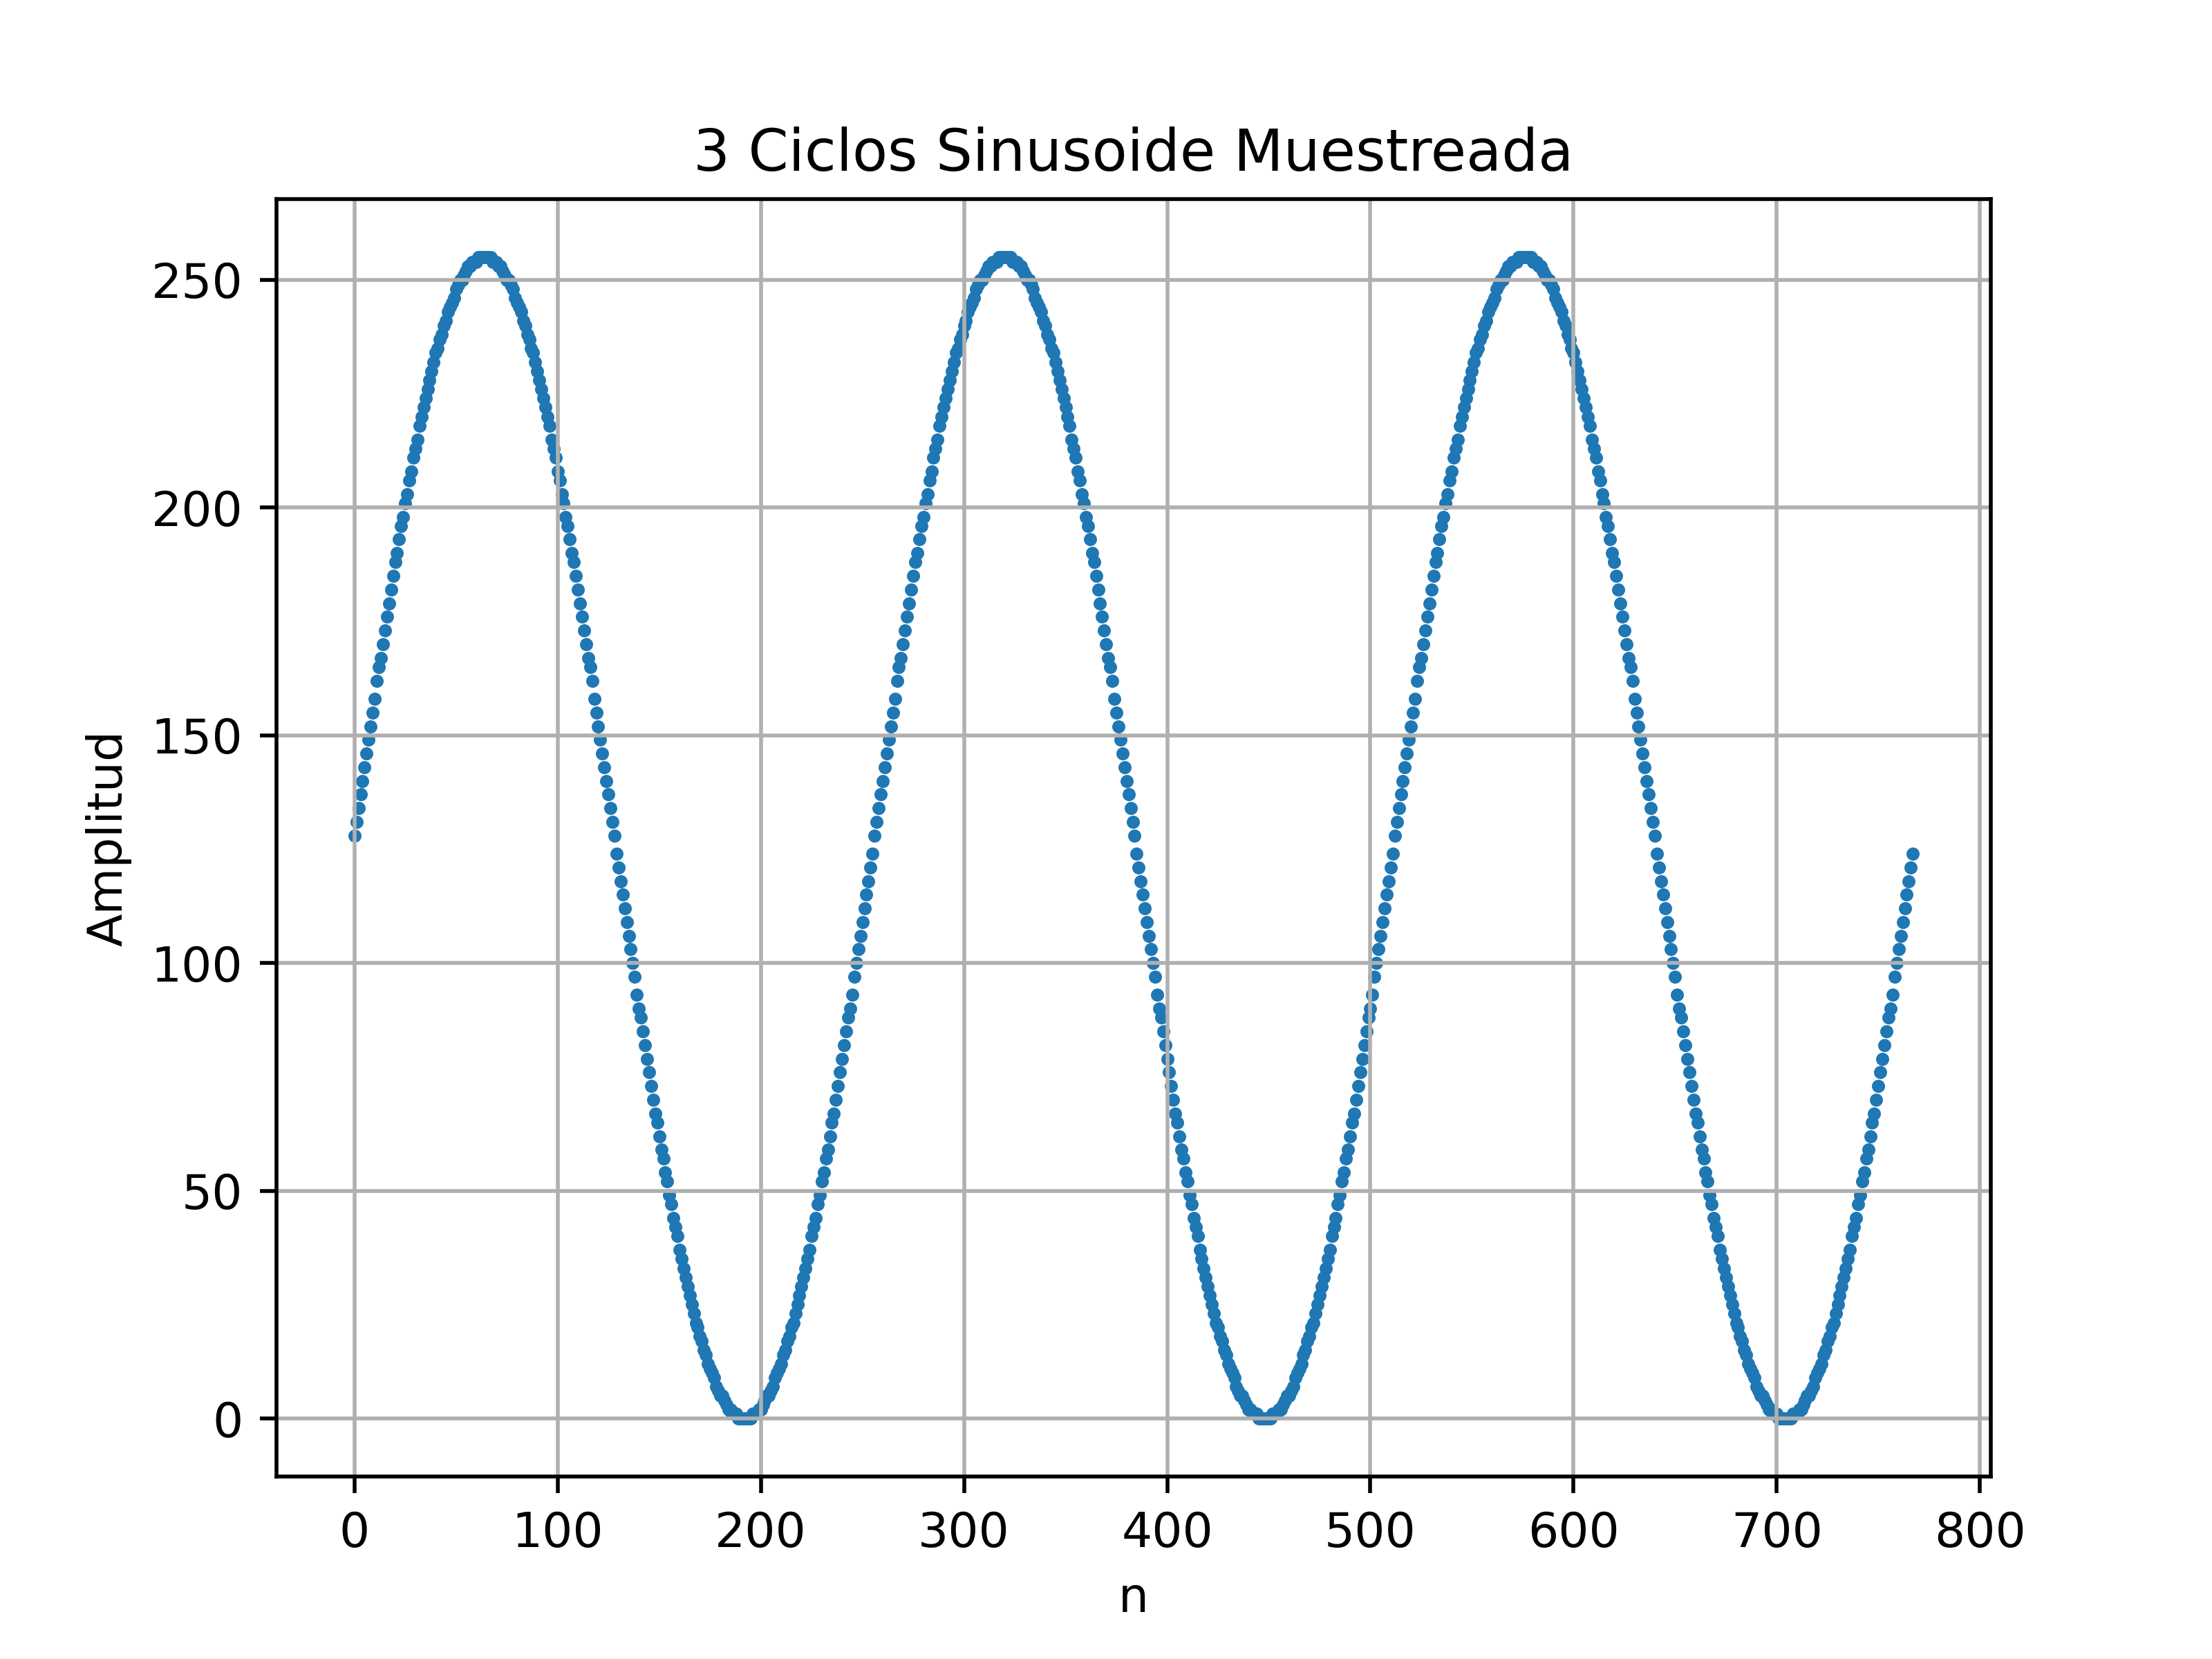
\includegraphics[width=0.8\textwidth]{Sinusoide_Muestreada.png}
    \caption{Tres ciclos consecutivos de la senoide cuantizada en 8 bits.}
\end{figure}
Para implementar la señal sinusoidal en la FPGA, se utilizó una memoria ROM de 256 posiciones, con palabras de 8 bits. Cada posición de memoria almacena una muestra de la señal sinusoidal generada previamente.

El archivo \texttt{sine.mem} se carga en la ROM mediante la instrucción \texttt{\$readmemh}, y la salida de la memoria depende de una dirección de 8 bits. De este modo, un contador puede recorrer secuencialmente las direcciones de la memoria y obtener un período completo de la senoide. Cuando el contador alcanza el valor 255 y vuelve a 0, la señal se repite de manera cíclica.
\begin{lstlisting}[language=Verilog, caption={Módulo ROM para la señal sinusoidal}]
module Onda_Sinusoidal (
    input  wire [7:0] addr,
    output wire [7:0] data
);

    reg [7:0] mem [0:255];

    initial begin
        $readmemh("sine.mem", mem);
    end

    assign data = mem[addr];

endmodule
\end{lstlisting}
Para validar el correcto funcionamiento del módulo implementado, se desarrolló un testbench en Verilog que recorre secuencialmente las direcciones de la memoria ROM. En particular, se simularon tres ciclos completos de la señal, correspondientes a 768 muestras.

La simulación permitió observar que la señal generada presenta la forma esperada de una sinusoide discreta y que la secuencia se repite correctamente cada 256 muestras. Esto confirma que el acceso cíclico a la memoria se realiza de manera adecuada y que no existen discontinuidades significativas entre ciclos consecutivos.
\begin{figure}[H]
    \centering
    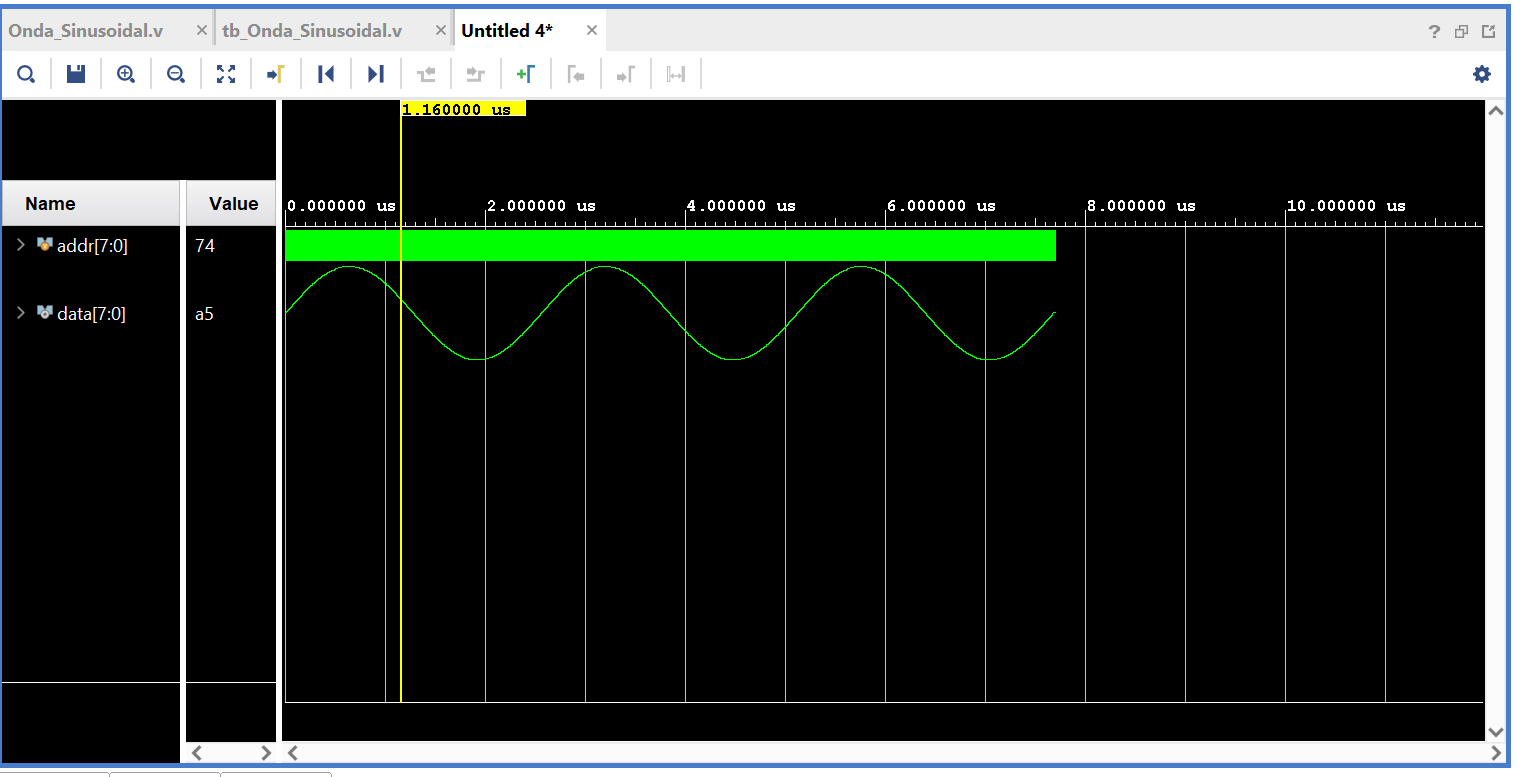
\includegraphics[width=0.9\textwidth]{tb_Sinusoide.png}
    \caption{Simulacion Vivado}
\end{figure}

2. Una forma de dividir la frecuencia del reloj consiste en utilizar un contador que genere una nueva señal periódica, la cual se utiliza como un reloj de menor frecuencia. En este método, el contador incrementa su valor en cada flanco de subida del reloj maestro y, al alcanzar un valor predefinido, cambia el estado de una señal de salida. Esta señal resultante (\texttt{clk\_div}) se utiliza como nuevo reloj para controlar otros bloques del sistema, por ejemplo mediante instrucciones del tipo \texttt{always @(posedge clk\_div)}. De esta forma, se crea un nuevo reloj más lento que define el ritmo de operación de parte del sistema.\\

\textbf{Ventajas:}
\begin{itemize}
    \item Implementación simple e intuitiva.
    \item Permite generar señales periódicas con ciclo útil cercano al 50\%.
\end{itemize}

\textbf{Desventajas:}
\begin{itemize}
    \item Introduce un nuevo dominio de reloj.
    \item Puede generar problemas de sincronización y \textit{skew}.
    \item Complica el análisis temporal del diseño.
    \item No siempre permite obtener exactamente la frecuencia deseada.
\end{itemize}

Otra forma de dividir la frecuencia consiste en mantener el reloj maestro único y generar una señal de habilitación, comúnmente llamada \textit{tick} o \textit{clock enable}. En este caso, también se utiliza un contador que incrementa con el reloj principal, pero en lugar de generar un nuevo reloj, produce un pulso breve cuando alcanza un valor determinado. Este pulso se utiliza como condición dentro de un bloque del tipo \texttt{always @(posedge clk) if (tick)} para actualizar los registros. De esta manera, el reloj no se modifica, sino que se controla la velocidad a la que operan los distintos módulos del sistema.\\

\textbf{Ventajas:}
\begin{itemize}
    \item Mantiene un único dominio de reloj.
    \item Evita problemas de sincronización.
    \item Es el método recomendado en FPGA.
    \item Permite controlar fácilmente la velocidad de operación de los módulos.
\end{itemize}

\textbf{Desventajas:}
\begin{itemize}
    \item No genera un reloj físico independiente.
    \item No es adecuado si se requiere una señal de reloj explícita para otros bloques.
\end{itemize}

En este proyecto se utiliza el segundo método, ya que permite controlar la velocidad de lectura de la memoria ROM sin introducir nuevos dominios de reloj.\\

3. El oscilador local fue implementado utilizando una arquitectura basada en una memoria ROM que almacena una señal sinusoidal discretizada, junto con un sistema de control que regula la velocidad a la que se recorren sus muestras. De esta forma, es posible generar señales periódicas de distintas frecuencias a partir de un único reloj maestro.\\

El sistema está compuesto por tres bloques principales:

\begin{itemize}
    \item Generador de señal de habilitación (\textit{clk\_mgmt})
    \item Contador
    \item Memoria ROM con la señal sinusoidal
\end{itemize}

El funcionamiento es el siguiente: el generador de habilitación produce un pulso periódico (\textit{tick}) que indica cuándo el contador debe avanzar. Este pulso se conecta directamente como señal de control del contador. Cada vez que el contador avanza, cambia la dirección que se está leyendo en la memoria ROM, y así se obtiene una nueva muestra de la señal sinusoidal. Al repetirse este proceso de forma continua, se genera una señal periódica.\\

El módulo \texttt{clk\_mgmt} tiene como objetivo dividir la frecuencia del reloj maestro utilizando un contador interno. Este contador es independiente del contador que recorre la memoria. En cada ciclo del reloj, este contador aumenta su valor hasta llegar a un número definido (\texttt{DIV}). Cuando alcanza ese valor, se genera un pulso (\textit{tick}) y el contador vuelve a cero.

Este pulso no es un nuevo reloj, sino una señal que indica cuándo el sistema debe actualizarse. De esta forma, todo el diseño sigue usando el mismo reloj, lo que evita problemas de sincronización.

El valor de \texttt{DIV} se selecciona mediante los switches de la placa, lo que permite cambiar la frecuencia de la señal generada.\\

El módulo \texttt{counter} corresponde a un segundo contador, distinto al anterior, cuya función es recorrer las direcciones de la memoria ROM. Este contador solo avanza cuando la señal \textit{tick} está activa, lo que permite controlar la velocidad a la que se leen las muestras.

Como el contador es de 8 bits, puede tomar valores entre 0 y 255. Al llegar al valor máximo, vuelve automáticamente a 0, lo que hace que la lectura de la memoria sea cíclica y, por lo tanto, que la señal generada sea periódica.\\

El módulo \texttt{Onda\_Sinusoidal} corresponde a una memoria ROM de 256 posiciones, donde cada posición contiene una muestra de una señal sinusoidal representada en 8 bits. Estas muestras fueron generadas previamente y guardadas en el archivo \texttt{sine.mem}.

La entrada de esta memoria es la dirección entregada por el contador, y su salida es la muestra correspondiente de la señal. De esta manera, al recorrer las direcciones una tras otra, se reconstruye la señal sinusoidal de forma discreta.\\

Cada período de la señal sinusoidal está compuesto por 256 muestras. Por lo tanto, la frecuencia de salida depende de la velocidad a la que se recorren estas muestras:

\[
f_{\text{salida}} = \frac{f_{\text{lectura}}}{256}.
\]

La frecuencia de lectura está determinada por el generador de habilitación, el cual produce un pulso cada \texttt{DIV} ciclos del reloj maestro. Por lo tanto:

\[
f_{\text{lectura}} = \frac{f_{clk}}{DIV}.
\]

Combinando ambas expresiones, se obtiene:

\[
f_{\text{salida}} = \frac{f_{clk}}{256 \cdot DIV}.
\]

Asumiendo un reloj maestro de 100 MHz, se calcularon los valores de \texttt{DIV} para obtener frecuencias cercanas a las especificadas en el enunciado.\\

Los valores utilizados y las frecuencias resultantes se muestran en la siguiente tabla:

\begin{center}
\begin{tabular}{c c c c}
\hline
\texttt{sw} & Frecuencia deseada & $DIV$ & Frecuencia obtenida \\
\hline
00 & 220.00 Hz & 1775 & 220.07 Hz \\
01 & 391.99 Hz & 997  & 391.80 Hz \\
10 & 554.36 Hz & 705  & 554.08 Hz \\
11 & 739.98 Hz & 528  & 739.82 Hz \\
\hline
\end{tabular}
\end{center}

Las pequeñas diferencias entre las frecuencias deseadas y las obtenidas se deben a que el valor de \texttt{DIV} debe ser un número entero. Como consecuencia, no siempre es posible obtener exactamente la frecuencia deseada, por lo que se utiliza el valor entero más cercano.\\

Veamos el resultado de la implementación del oscilador local en la FPGA. En la figura se observa el comportamiento del sistema, donde se evidencia la generación de la señal sinusoidal discreta y la variación de su frecuencia en función de los switches de selección.
\begin{figure}[H]
    \centering
    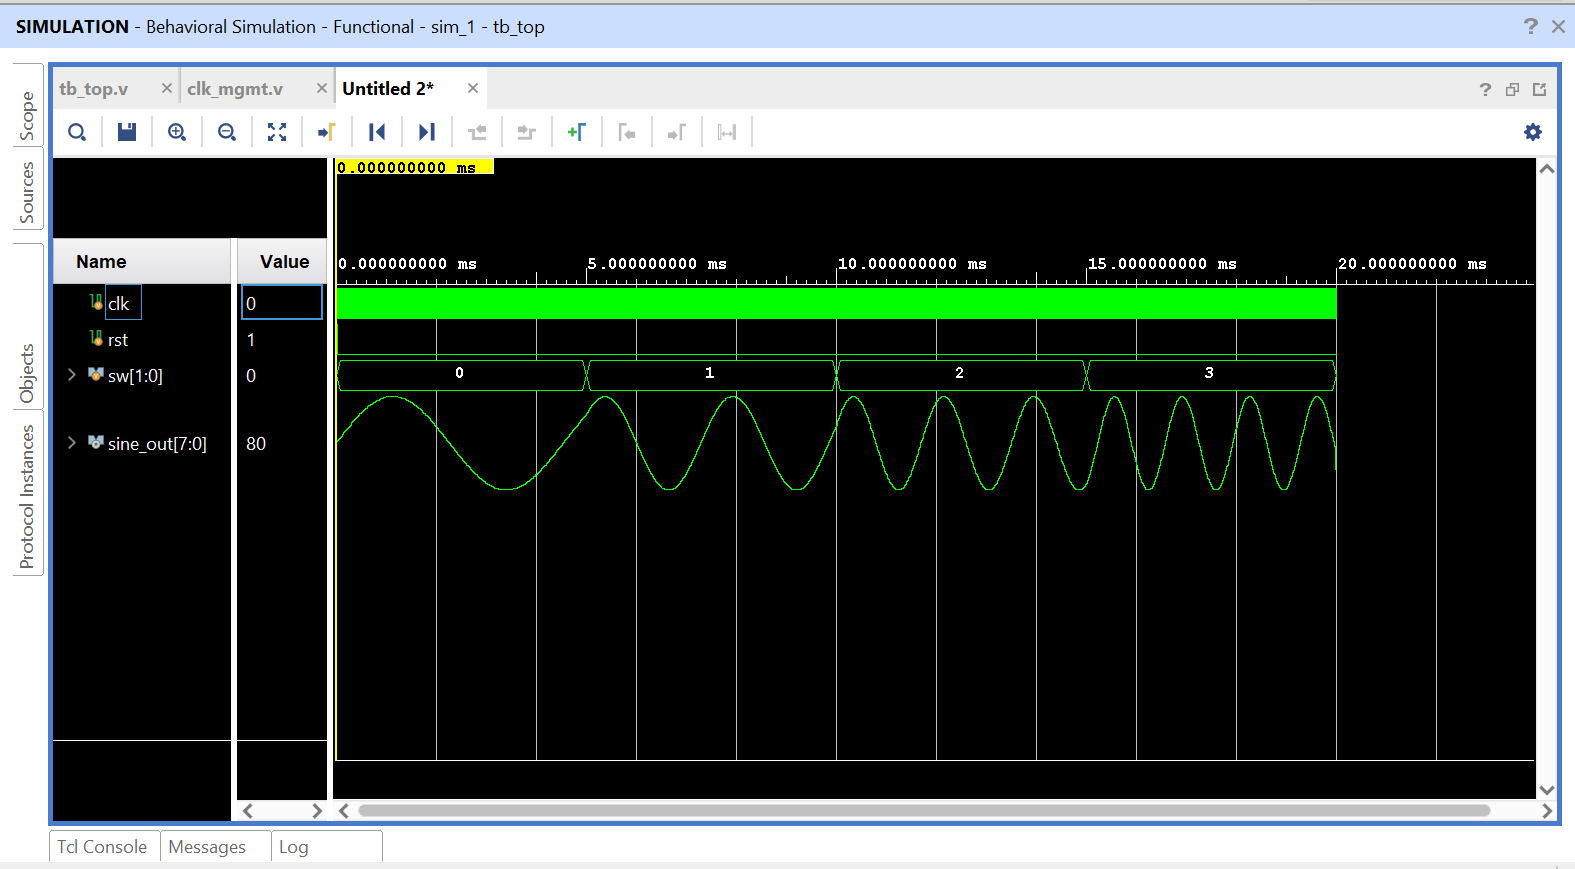
\includegraphics[width=0.9\textwidth]{tb_top.png}
    \caption{Resultado de la implementación}
\end{figure}

4. Para implementar el modulador PWM se utiliza un contador de 8 bits que genera una señal tipo diente de sierra, recorriendo los valores entre 0 y 255 de forma cíclica:

\[
0 \to 1 \to 2 \to \dots \to 255 \to 0
\]

Como el contador recorre 256 valores por período, para obtener una señal de 25 kHz la frecuencia de conteo debe ser:

\[
f_{\text{count}} = 256 \cdot 25\,000 = 6\,400\,000 \text{ Hz}
\]

Por lo tanto, la frecuencia a la que debe contar el contador es:

\[
\boxed{f_{\text{count}} = 6.4\ \text{MHz}}
\]

Asumiendo un reloj maestro de 100 MHz, el divisor requerido sería:

\[
DIV = \frac{100\,000\,000}{6\,400\,000} = 15.625
\]

Como este valor no es entero, no es posible obtener exactamente dicha frecuencia usando un divisor entero simple en Verilog. Por ello, se escoge el valor entero más cercano. En este caso, una buena aproximación es \(DIV=16\), lo que entrega una frecuencia de conteo de:

\[
f_{\text{count, real}} = \frac{100\,000\,000}{16} = 6.25\ \text{MHz}
\]

y, por lo tanto, una frecuencia real para la señal diente de sierra de:

\[
f_{\text{sierra, real}} = \frac{6.25\ \text{MHz}}{256} \approx 24.41\ \text{kHz}
\]

La diferencia respecto a los 25 kHz deseados se debe a que el método de división utilizado trabaja con divisores enteros, por lo que no siempre es posible obtener exactamente la frecuencia requerida.
\end{document}